\documentclass{article}
\usepackage{fullpage}
\usepackage{latexsym}
\usepackage{amsfonts}
\usepackage{amssymb}
\usepackage{graphicx}
\usepackage{amsmath}
\usepackage{bbm}

\title{AMATH 583 Homework 1}
\author{Lucas Cassin Cruz Burke}

\begin{document}

\maketitle

\section*{Problem 1}
I used a C++ program to find a practical measure of my machines SP (32 bit) and DP (64 bit) precision by taking the difference of two numbers and comparing the result to zero in each data type. 
\begin{itemize}
    \item Single point (32-bit) precision: 24 bits 
    \item Double point (64 bit) precision: 53 bits
\end{itemize}

\section*{Problem 2}

In the IEEE floating-point standard we represent numbers using a sign bit, an exponent, and a mantissa, as shown. $$x = \pm \left( d_0 + \frac{d_1}{\beta} + \frac{d_2}{\beta^2} + \dots + \frac{d_{p-1}}{\beta^{p-1}}\right)\beta^E$$

For SP (32 bit) numbers the IEEE standard utilizes one sign bit, eight exponent bits, and 23 mantissa bits. The exponent is biased, with a bias of $2^{8}/2-1=127$. Note that all ones is reserved for representing $\pm \infty$, hence the largest exponent value is 11111110, which is 254 in decimal, which represents an unbiased exponent of $254-127=127$. To find the largest SP number we let the sign bit equal zero, and set the mantissa to be all ones. Likewise, to find the smallest (most negative) SP number, we let the sign bit equal one to switch our number to a negative. Therefore, the largest SP number which can be represented in IEEE is 

$$(-1)^0 \cdot \left(1 + 2^{-1} + 2^{-2} + \dots + 2^{-23} \right)\cdot 2^{127} \approx 3.402 \times 10^{38}$$

while the smallest (most negative) SP number is given by 

$$(-1)^1 \cdot \left(1 + 2^{-1} + 2^{-2} + \dots + 2^{-23} \right)\cdot 2^{127} \approx -3.402 \times 10^{38}$$

For DP (64 bit) numbers we have one sign bit, eleven exponent bits, and 52 mantissa bits. Similar to above, the largest available exponent is 11111111110 (2046 in decimal), which represents an unbiased exponent of 2046 - 1023 = 1023. Hence, in line with the above reasoning for the SP case, the largest DP number which can be represented is given by 

$$(-1)^0 \cdot \left(1 + 2^{-1} + 2^{-2} + \dots + 2^{-52} \right)\cdot 2^{1023} \approx 1.797 \times 10^{308}$$

while the smallest (most negative) DP number is given by

$$(-1)^0 \cdot \left(1 + 2^{-1} + 2^{-2} + \dots + 2^{-52} \right)\cdot 2^{1023} \approx -1.797 \times 10^{308}.$$

\section*{Problem 3}

When we multiply $200 \times 300 \times 400 \times 500$ using the integer type in C++ we receive the result -884901888. This is due to overflow: integers in C++ are by default represented using 32 bits, one of which is a sign bit, which gives a maximum integer representation of 2,147,483,647. Since $200 \times 300 \times 400 \times 500=12,000,000,000$ is larger than the maximum representable integer the resulting value "wraps around" the representable range, and the stored result is incorrect. 

\begin{itemize}
    \item \textbf{Overflow:} Overflow occurs when the result of an operation is too large to be represented by the specific data type being used. The resulting number "wraps around" the representable range, which can lead to large positive numbers being erroneously stored as negative numbers, for example. 
    \item \textbf{Underflow:} Underflow is a term more commonly associated with floating-point numbers and is not directly applicable to integer data types. It occurs when the result of a floating-point operation is too small (close to zero) to be represented by the smallest representable positive normal number in the floating-point format. In this situation the result will either be rounded down to the smallest representable positive subnormal number (zero), or cause an underflow exception.
\end{itemize}

\section*{Problem 4}
To find the number of normalized floating-point numbers for Single Precision (SP) and Double Precision (DP) representations, we need to consider the number of possible combinations of exponent and mantissa values, excluding the reserved exponent values for special numbers (subnormal, infinity, and NaN).

\begin{enumerate}
    \item \textbf{SP - 32-bit}: \begin{itemize}
        \item Sign: 1 bit ($2^1=2$ possible values).
        \item Exponent: 8 bits ($2^8 = 256$ possible values). We exclude two reserved exponent values (all 0s and all 1s), leaving 254 usable exponent values.
        \item Mantissa: 23 bits ($2^{23} = 8,388,608$ possible values). For normalized numbers, the leading digit is always assumed to be 1, so we only need to consider the remaining 22 bits for the fractional part of the mantissa.
    \end{itemize} 
    Considering both the positive and negative numbers, the total number of SP normalized floating-point numbers is: $$2 \times 254 \times 8,388,608 \approx 4.278 \times 10^9$$

    \item \textbf{DP - 64-bit:} \begin{itemize}
        \item Sign: 1 bit ($2^1=2$ possible values).
        \item Exponent: 11 bits ($2^{11} = 2,048$ possible values). We exclude two reserved exponent values (all 0s and all 1s), leaving 2,046 usable exponent values.
        \item Mantissa: 52 bits ($2^{52} \approx 4.503 \times 10^{15}$ possible values). For normalized numbers, the leading digit is always assumed to be 1, so we only need to consider the remaining 51 bits for the fractional part of the mantissa.
    \end{itemize}
    Considering both the positive and negative numbers, the total number of DP normalized floating-point numbers is: $$2 \times 2,046 \times 4.503 \times 10^{15} \approx 1.844 \times 10^{19}$$

    In summary: 

    \begin{itemize}
        \item There are approximately $4.278 \times 10^9$ normalized Single Precision (32-bit) floating-point numbers.
        \item There are approximately $1.844 \times 10^{19}$ normalized Double Precision (64-bit) floating-point numbers.
    \end{itemize}
\end{enumerate}

\section*{Problem 5}
We consider a 6-bit floating point system consisting of one sign bit ($s=1$), a 3-bit exponent ($k=3$), and a 2-bit mantissa ($n=2$). 

For normalized numbers, we have numbers of the form $$(-1)^s \times 1.m \times 2^{e-\text{bias}}$$

We enumerate all of the possible 6-bit floating point numbers below. 

\subsection*{Normalized}
Normalized values have an exponent $E \ne 000$, and the fractional part $f$ has an implicit leading 1 which is added to the mantissa decimal.

\begin{tabular}{|c|c|c|c|c|c|}
    \hline
    Sign bit (S) & Exponent bits (E) & Mantissa Bits (M) & Exponent decimal & Mantissa decimal & Decimal Value \\
    \hline
    0 & 001 & 00 & -2 & 0 & 1/4 \\
    0 & 001 & 01 & -2 & 1/4 & 5/16 \\
    0 & 001 & 10 & -2 & 1/2 & 3/8 \\
    0 & 001 & 11 & -2 & 3/4 & 7/16 \\
    0 & 010 & 00 & -1 & 0 & 1/2 \\
    0 & 010 & 01 & -1 & 1/4 & 5/8 \\
    0 & 010 & 10 & -1 & 1/2 & 3/4 \\
    0 & 010 & 11 & -1 & 3/4 & 7/8 \\
    0 & 011 & 00 & 0 & 0 & 1 \\
    0 & 011 & 01 & 0 & 1/4 & 5/4 \\
    0 & 011 & 10 & 0 & 1/2 & 3/2 \\
    0 & 011 & 11 & 0 & 3/4 & 7/4 \\
    0 & 100 & 00 & 1 & 0 & 2 \\
    0 & 100 & 01 & 1 & 1/4 & 5/2 \\
    0 & 100 & 10 & 1 & 1/2 & 3 \\
    0 & 100 & 11 & 1 & 3/4 & 7/2 \\
    0 & 101 & 00 & 2 & 0 & 1 \\
    0 & 101 & 01 & 2 & 1/4 & 5 \\
    0 & 101 & 10 & 2 & 1/2 & 3 \\
    0 & 101 & 11 & 2 & 3/4 & 7 \\
    0 & 110 & 00 & 3 & 0 & 2 \\
    0 & 110 & 01 & 3 & 1/4 & 10 \\
    0 & 110 & 10 & 3 & 1/2 & 6 \\
    0 & 110 & 11 & 3 & 3/4 & 14 \\
    1 & 001 & 00 & -2 & 0 & -1/4 \\
    1 & 001 & 01 & -2 & 1/4 & -5/16 \\
    1 & 001 & 10 & -2 & 1/2 & -3/8 \\
    1 & 001 & 11 & -2 & 3/4 & -7/16 \\
    1 & 010 & 00 & -1 & 0 & -1/2 \\
    1 & 010 & 01 & -1 & 1/4 & -5/8 \\
    1 & 010 & 10 & -1 & 1/2 & -3/4 \\
    1 & 010 & 11 & -1 & 3/4 & -7/8 \\
    1 & 011 & 00 & 0 & 0 & -1 \\
    1 & 011 & 01 & 0 & 1/4 & -5/4 \\
    1 & 011 & 10 & 0 & 1/2 & -3/2 \\
    1 & 011 & 11 & 0 & 3/4 & -7/4 \\
    1 & 100 & 00 & 1 & 0 & -2 \\
    1 & 100 & 01 & 1 & 1/4 & -5/2 \\
    1 & 100 & 10 & 1 & 1/2 & -3 \\
    1 & 100 & 11 & 1 & 3/4 & -7/2 \\
    1 & 101 & 00 & 2 & 0 & -1 \\
    1 & 101 & 01 & 2 & 1/4 & -5 \\
    1 & 101 & 10 & 2 & 1/2 & -3 \\
    1 & 101 & 11 & 2 & 3/4 & -7 \\
    1 & 110 & 00 & 3 & 0 & -2 \\
    1 & 110 & 01 & 3 & 1/4 & -10 \\
    1 & 110 & 10 & 3 & 1/2 & -6 \\
    1 & 110 & 11 & 3 & 3/4 & -14 \\
    \hline
\end{tabular}

\subsection*{Denormalized}

Denormalized numbers all have an exponent of $E=000$, and the fractional part has no implicit leading order 1. Denormalized numbers in this case implicitely have an exponent value of $E=-2$. The denormalized 6-bit floating point numberes are enumerated below. 

\begin{tabular}{|c|c|c|c|}
    \hline
    Sign bit (S) & Mantissa Bits (M) & Mantissa decimal & Decimal Value \\
    \hline
    0 & 00  & 0 & +0 \\
    0 & 01  & 1/4 & 1/16 \\
    0 & 10  & 1/2 & 1/8 \\
    0 & 11  & 3/4 & 3/16 \\
    1 & 00  & 0 & -0 \\
    1 & 01  & 1/4 & -1/16 \\
    1 & 10  & 1/2 & -1/8 \\
    1 & 11  & 3/4 & -3/16 \\
    \hline
\end{tabular}

\subsection*{Distribution of representable numbers}
Lastly, below is a figure showing the location of all of the above representable 6-bit floating point numbers on the number line. 

\begin{figure}[h]
    \centering
    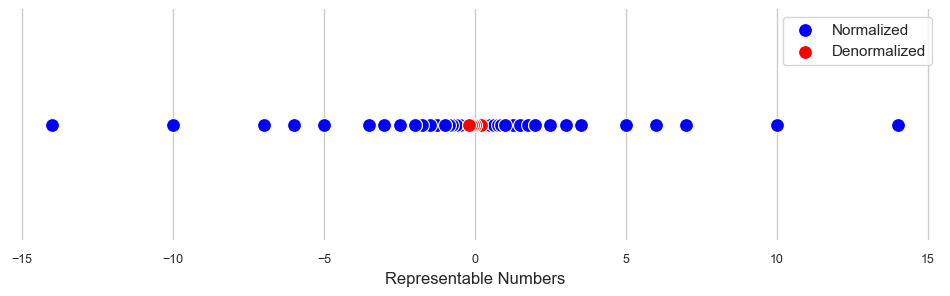
\includegraphics[scale=0.7]{RepresentableNumbers.png}
    \caption{Number line plot of representable 6-bit numbers.}
    \label{fig:representable-numbers}
  \end{figure}
  

\end{document}
